\section{Specific requirements}

\subsection{External interfaces}
%----------------------------------------------------------------------
\begin{tabular}{ll}
%--------------------------------
\textbf{Found in requirement}&Add User Account : FRQ1\\
\textbf{Name of item}&Username\\
\textbf{Description of purpose}&The desired Username which the application\\& authenticates the user\\
\textbf{Source of input}&User\\
\textbf{Destination of output}&Application database\\
\textbf{Valid range, accuracy, and/or tolerance}&Standard GSM 03.38 character set\\
\textbf{Relationships to other inputs/outputs}&A user account will be bound to the\\& desired username provided by the user\\
&\\
&\\
%--------------------------------
\textbf{Found in requirement}&Add User Account : FRQ1\\
\textbf{Name of item}&Password\\
\textbf{Description of purpose}&The desired password which will be associated\\& with the specific username created by\\& the user\\
\textbf{Source of input}&User\\
\textbf{Destination of output}&Application database\\
\textbf{Valid range, accuracy, and/or tolerance}&Standard GSM 03.38 character set\\
\textbf{Relationships to other inputs/outputs}&A user account will have the password\\& associated with the provided username\\& set by the user to this value\\
&\\
&\\
%--------------------------------
\textbf{Found in requirement}&Add User Account : FRQ1\\
\textbf{Name of item}&Password Confirmation\\
\textbf{Description of purpose}&A prompt to re-enter the password\\& provided by the user\\
\textbf{Source of input}&User\\
\textbf{Destination of output}&N/A\\
\textbf{Valid range, accuracy, and/or tolerance}&Standard GSM 03.38 character set\\
\textbf{Relationships to other inputs/outputs}&The value submitted is used to confirm the\\& correctness of the desired password by the user\\& in order to accommodate for human\\& error\\
&\\
&\\
%--------------------------------
\textbf{Found in requirement}&Add User Account : FRQ1\\
\textbf{Name of item}&User Account\\
\textbf{Description of purpose}&The user account that has been created and has\\& been associated with the provided username\\& and password submitted by the user\\
\textbf{Source of input}&Application\\
\textbf{Destination of output}&Application database\\
\textbf{Valid range, accuracy, and/or tolerance}&Checked during creation process\\
\textbf{Relationships to other inputs/outputs}&The username and password entered by\\& the user in order to create the sole account\\& linked to the application\\
&\\
&\\
%--------------------------------
\end{tabular}
%--------------------------------
\newpage
\begin{tabular}{ll}
%--------------------------------
\textbf{Found in requirement}&Add User Account : FRQ1\\
\textbf{Name of item}&Error Message\\
\textbf{Description of purpose}&This message indicates that an error has been\\& found during account creation, and that,\\& accordingly, no account has been created\\
\textbf{Source of input}&Application error checking\\
\textbf{Destination of output}&User interface\\
\textbf{Valid range, accuracy, and/or tolerance}&N/A\\
\textbf{Relationships to other inputs/outputs}&The details provided during account creation\\& was invalid for one or more reasons\\
&\\
%--------------------------------
\textbf{Found in requirement}&Local Authentication : FRQ3\\
\textbf{Name of item}&Username\\
\textbf{Description of purpose}&The username associated with the user account\\& that the user logs into the application with\\
\textbf{Source of input}&User\\
\textbf{Destination of output}&N/A\\
\textbf{Valid range, accuracy, and/or tolerance}&Standard GSM 03.38 character set\\
\textbf{Relationships to other inputs/outputs}&The username that was used to create\\& the user account\\
&\\
%--------------------------------
\textbf{Found in requirement}&Local Authentication : FRQ3\\
\textbf{Name of item}&Password\\
\textbf{Description of purpose}&The password associated with the user account\\& that the user logs into the application with\\
\textbf{Source of input}&User\\
\textbf{Destination of output}&N/A\\
\textbf{Valid range, accuracy, and/or tolerance}&Standard GSM 03.38 character set\\
\textbf{Relationships to other inputs/outputs}&The password that was provided by the\\& user in order to create the user account\\
&\\
%--------------------------------
\textbf{Found in requirement}&Local Authentication : FRQ3\\
\textbf{Name of item}&Error Message\\
\textbf{Description of purpose}&The error message informs the user that the\\& authentication process failed\\
\textbf{Source of input}&Application logic\\
\textbf{Destination of output}&User interface\\
\textbf{Valid range, accuracy, and/or tolerance}&N/A\\
\textbf{Relationships to other inputs/outputs}&The username and password provided during the login phase\\& don't correlate with the user account that has\\& been created on the device\\
&\\
%--------------------------------
\end{tabular}
%--------------------------------
\newpage
%--------------------------------
\begin{tabular}{ll}
%--------------------------------
\textbf{Found in requirement}&Add Contact : FRQ10\\
\textbf{Name of item}&Contact Name\\
\textbf{Description of purpose}&The name a user wishes to have associated with\\& the intended receiver of future messages\\
\textbf{Source of input}&User\\
\textbf{Destination of output}&User interface\\
\textbf{Valid range, accuracy, and/or tolerance}&Any character data\\
\textbf{Relationships to other inputs/outputs}&The text entered by the user to represent a specific\\& contact on the device\\
&\\
%--------------------------------
\textbf{Found in requirement}&Add Contact : FRQ10\\
\textbf{Name of item}&Contact Number\\
\textbf{Description of purpose}&The mobile phone number associated with the contact\\& being added to the device\\
\textbf{Source of input}&Contact\\
\textbf{Destination of output}&N/A\\
\textbf{Valid range, accuracy, and/or tolerance}&Standard mobile phone numbers\\&with or without the international dialing prefix\\
\textbf{Relationships to other inputs/outputs}&The value entered by the user to represent\\& a contact's mobile phone number\\& , and is associated with the provided contact\\& name\\
&\\
%--------------------------------
\textbf{Found in requirement}&Add Contact : FRQ10\\
\textbf{Name of item}&Local Key\\
\textbf{Description of purpose}&The key generated locally which will be\\& used by the application encryption algorithm\\
\textbf{Source of input}&Application generated; user initiated\\
\textbf{Destination of output}&N/A\\
\textbf{Valid range, accuracy, and/or tolerance}&Standard GSM 03.38 character set\\
\textbf{Relationships to other inputs/outputs}&This key will be used in conjunction with\\& the key generated by the contact to ensure synchronization,\\& and therefore secure communication, between the\\& two synchronized devices\\
&\\
%--------------------------------
\textbf{Found in requirement}&Add Contact : FRQ10\\
\textbf{Name of item}&Contact Key\\
\textbf{Description of purpose}&The key generated locally by the contact which\\& will be used by the application encryption algorithm\\
\textbf{Source of input}&Contact\\
\textbf{Destination of output}&N/A\\
\textbf{Valid range, accuracy, and/or tolerance}&Standard GSM 03.38 character set\\
\textbf{Relationships to other inputs/outputs}&This key will be used in conjunction with\\& the locally generated key to ensure synchronization,\\& and therefore secure communication, between the\\& two synchronized devices\\
&\\
%--------------------------------
\textbf{Found in requirement}&Add Contact : FRQ10\\
\textbf{Name of item}&Contact\\
\textbf{Description of purpose}&The contact that has been created\\
\textbf{Source of input}&Application\\
\textbf{Destination of output}&Application database\\
\textbf{Valid range, accuracy, and/or tolerance}&N/A\\
\textbf{Relationships to other inputs/outputs}&All entered contact details are validated\\& and stored in the applciation's local database\\
&\\
%--------------------------------
\end{tabular}
%--------------------------------
\newpage
%--------------------------------
\begin{tabular}{ll}
%--------------------------------
\textbf{Found in requirement}&Add Contact : FRQ10\\
\textbf{Name of item}&Error Message\\
\textbf{Description of purpose}&The error message informs the user that the\\& contact could not be added to the database\\
\textbf{Source of input}&Application logic\\
\textbf{Destination of output}&Application interface\\
\textbf{Valid range, accuracy, and/or tolerance}&N/A\\
\textbf{Relationships to other inputs/outputs}&The contact details that had been entered\\& by the user was found invalid\\
&\\
%--------------------------------
\textbf{Found in requirement}&Edit Contact : FRQ11\\
\textbf{Name of item}&Contact\\
\textbf{Description of purpose}&The selected contact to be edited by the user\\
\textbf{Source of input}&User\\
\textbf{Destination of output}&N/A\\
\textbf{Valid range, accuracy, and/or tolerance}&N/A\\
\textbf{Relationships to other inputs/outputs}&The selected contact's details stored in the\\& application database\\
&\\
%--------------------------------
\textbf{Found in requirement}&Edit Contact : FRQ11\\
\textbf{Name of item}&Local Key\\
\textbf{Description of purpose}&The key generated locally for device\\& resynchronization\\
\textbf{Source of input}&Application generated; user initiated\\
\textbf{Destination of output}&N/A\\
\textbf{Valid range, accuracy, and/or tolerance}&\\
\textbf{Relationships to other inputs/outputs}&This key will be used in conjunction with\\& the key generated by the contact to ensure resynchronization,\\& and therefore secure communication, between the\\& two synchronized devices\\
&\\
%--------------------------------
\textbf{Found in requirement}&Edit Contact : FRQ11\\
\textbf{Name of item}&Contact Key\\
\textbf{Description of purpose}&The key generated locally by the contact\\& for device resynchronization\\
\textbf{Source of input}&Contact\\
\textbf{Destination of output}&N/A\\
\textbf{Valid range, accuracy, and/or tolerance}&\\
\textbf{Relationships to other inputs/outputs}&This key will be used in conjunction with\\& the locally generated key to ensure resynchronization,\\& and therefore secure communication, between the\\& two synchronized devices\\\\
&\\
%--------------------------------
\textbf{Found in requirement}&Edit Contact : FRQ11\\
\textbf{Name of item}&Contact\\
\textbf{Description of purpose}&The contact that has been updated\\
\textbf{Source of input}&N/A\\
\textbf{Destination of output}&Application database\\
\textbf{Valid range, accuracy, and/or tolerance}&N/A\\
\textbf{Relationships to other inputs/outputs}&All details related to the specific contact\\
&\\
%--------------------------------
\end{tabular}
%--------------------------------
\newpage
%--------------------------------
\begin{tabular}{ll}
%--------------------------------
\textbf{Found in requirement}&Edit Contact : FRQ11\\
\textbf{Name of item}&Error Message\\
\textbf{Description of purpose}&The error message informs the user that saving\\& the contact's edited data has been unsuccessful\\
\textbf{Source of input}&Application logic\\
\textbf{Destination of output}&Application interface\\
\textbf{Valid range, accuracy, and/or tolerance}&N/A\\
\textbf{Relationships to other inputs/outputs}&The contact details that had been\\& entered by the user was found to be invalid\\
&\\
%--------------------------------
\end{tabular}
%--------------------------------
%----------------------------------------------------------------------

\subsection{Functions}
\subsubsection{Admin Functions}
\begin{itemize}
\item{Add User Account : FRQ1}\\
\textbf{(Source: Bernard Wagner, Priority: Medium)}
\begin{itemize}
\item A user must be able to create a password protected account for the application
\item \textbf{Inputs:} The user enters a desired username, and password (as well as the password confirmation)
\item \textbf{Outputs:} A user account is either created and stored in the application database, or an error message is displayed and no account is created
\end{itemize}
 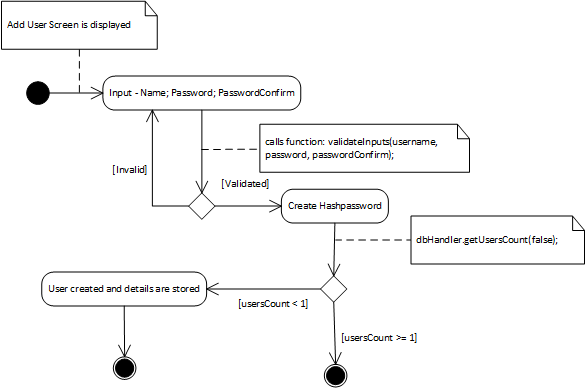
\includegraphics[width=13cm]{diagrams/StateDiagrams/AddUserStateDiagram.png}
\item{Edit User Account : FRQ2}\\
\textbf{(Source: Group Deliberation, Priority: Medium)}
\begin{itemize}
\item The user must be able to edit his/her user account details
\end{itemize}
 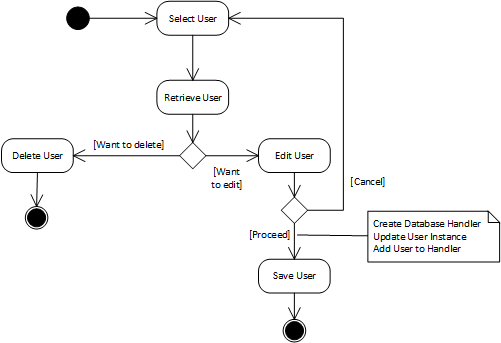
\includegraphics[width=13cm]{diagrams/StateDiagrams/EditUserStateDiagram.png}
\item{Local Authentication : FRQ3}\\%meaning functional requirement 3
\textbf{(Source: Bernard Wagner, Priority: Medium)}
\begin{itemize}
\item To ensure confidentiality, the application must authenticate a user by requiring a password before granting access to the application features
\item \textbf{Inputs:} The user enters his/her username and password
\item \textbf{Outputs:} After user authenticaion has been successful (the username/password provided had been found correct), access is granted to all application features. If authentication fails(and incorrect username/password was entered), and error message is displayed. If authentication fails repeatedly for a specific amount of times; within a specific time slot, the application is locked for a specific amount of time
\end{itemize}
 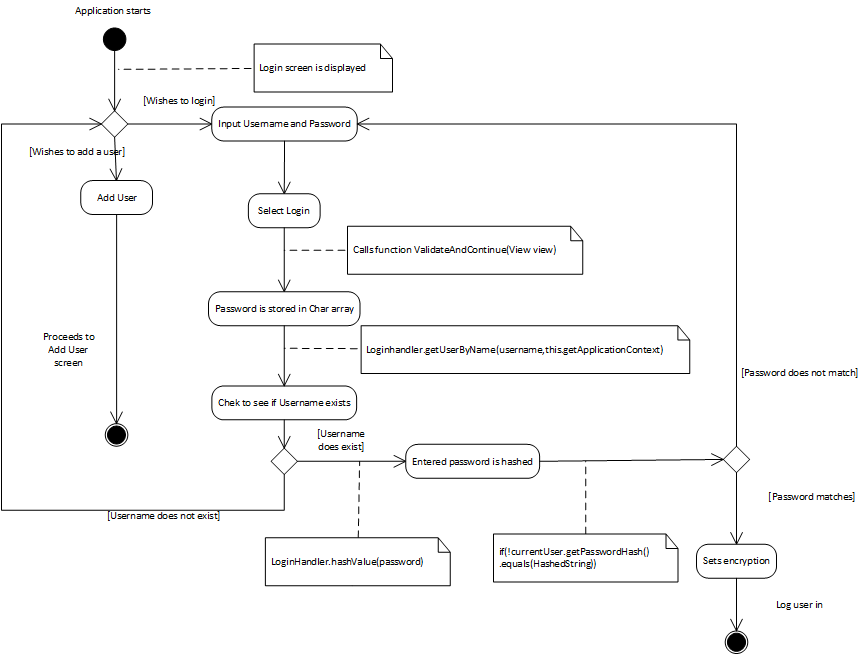
\includegraphics[width=13cm]{diagrams/StateDiagrams/LocalAuthenticationStateDiagram.png}
\end{itemize}
\subsubsection{Messaging Functions}
\begin{itemize}
\item{Enter message : FRQ4}\\%meaning functional requirement 1
\textbf{(Source: Bernard Wagner, Priority: High)}
\begin{itemize}
\item A user must be able to input text into the application
\end{itemize}
 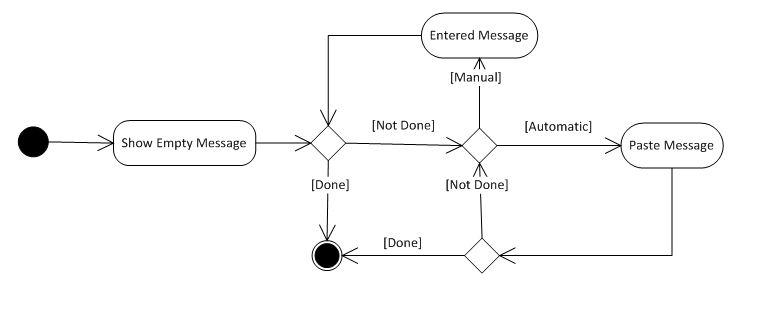
\includegraphics[width=13cm]{diagrams/StateDiagrams/EnterMessageState.png}
\item{Type message : FRQ4.1}\\
\textbf{(Source: Bernard Wagner, Priority: High)}
\begin{itemize}
\item A user must be able to type text into the application directly
\end{itemize}
\item{Paste message : FRQ4.2}\\
\textbf{(Source: Bernard Wagner, Priority: High)}
\begin{itemize}
\item A user must be able to paste an already constructed message into the application, using the device clipboard
\end{itemize}
\item{Edit Message: FRQ5}\\
\textbf{(Source: Bernard Wagner, Priority: Medium)}
\begin{itemize}
\item The message text must be editable once it has been input into the application
\end{itemize}
 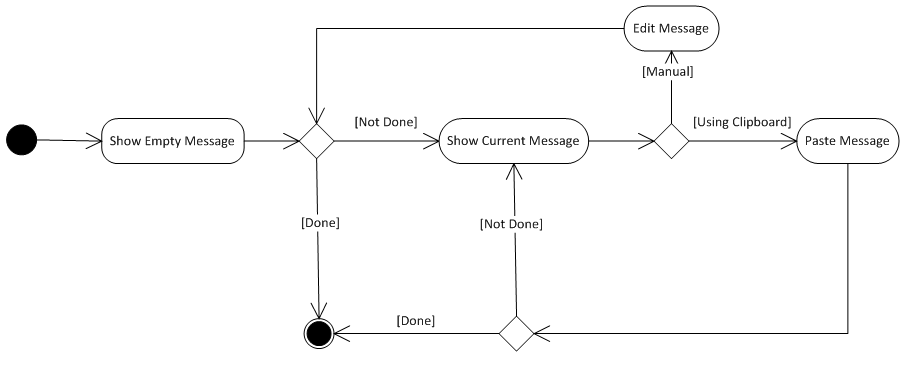
\includegraphics[width=13cm]{diagrams/StateDiagrams/EditMessageState.png}
\item{Encrypt message : FRQ6}\\
\textbf{(Source: Bernard Wagner, Priority: High)}
\begin{itemize}
\item The message must be encrypted using a suitable encryption method
\end{itemize}
 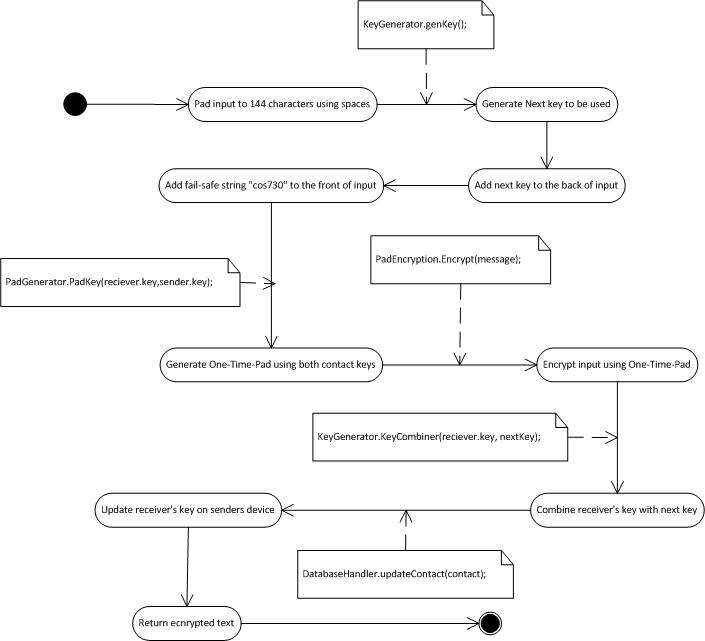
\includegraphics[width=13cm]{diagrams/StateDiagrams/EncryptMessageStateDiagram.png}
\item{Copy Encrypted Message : FRQ7}\\
\textbf{(Source: Bernard Wagner, Priority: High)}
\begin{itemize}
\item Once a message has been encrypted, a user must be able to copy the ciphertext, and paste it into any selected messaging application
\end{itemize}
\item{Decrypt message : FRQ8}\\
\textbf{(Source: Bernard Wagner, Priority: High)}
\begin{itemize}
\item The application must be able to decrypt received messages to reveal their original plaintext - if the sender of the message's contact is provided and synchronized
\end{itemize}
 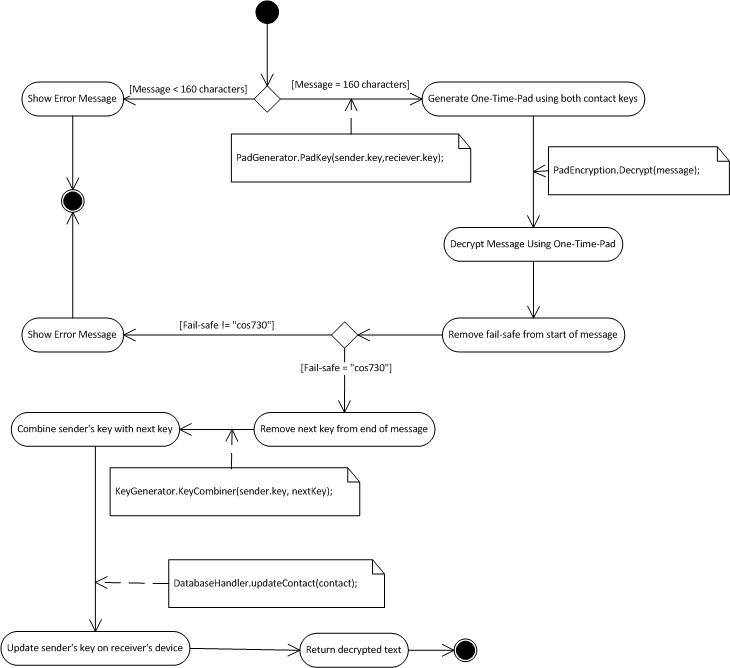
\includegraphics[width=13cm]{diagrams/StateDiagrams/DecryptMessageStateDiagram.png}
\item{Display message length : FRQ9}\\
\textbf{(Source: Bernard Wagner, Priority: Low)}
\begin{itemize}
\item The numbers of characters in a message must be displayed within the application
\end{itemize}
 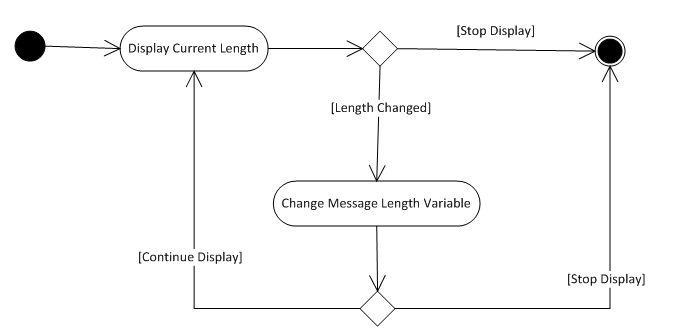
\includegraphics[width=13cm]{diagrams/StateDiagrams/DisplayMessageLengthState.png}
\end{itemize}
\subsubsection{Contacts Functions}
\begin{itemize}
\item{Add Contact : FRQ10}\\
\textbf{(Source: Bernard Wagner, Priority: High)}
\begin{itemize}
\item Before communicating with another user, the receiver of these (future) messages must be added as a contact on the local device, in order to be able to communicate with that user
\item \textbf{Inputs:} The receiver's name, mobile number, and locally generated key must be provided (along with the local device's generated key)
\item \textbf{Outputs:} The contact is created and stored in the application database, or the apllication displays an error message if the contact's details entered was found incorrect
\end{itemize}
 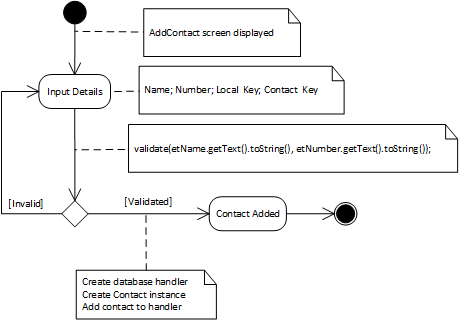
\includegraphics[width=13cm]{diagrams/StateDiagrams/AddContactStateDiagram.png}
\item{Edit Contact : FRQ11}\\
\textbf{(Source: Bernard Wagner, Priority: Medium)}
\begin{itemize}
\item A contact must be editable/deletable once it has been added
\item \textbf{Inputs:} The user selects a contact which they wish to modify, or delete, within the application
\item \textbf{Outputs:} The selected contact's details will be modified in the application database, or the contact will be removed from the application database
\end{itemize}
 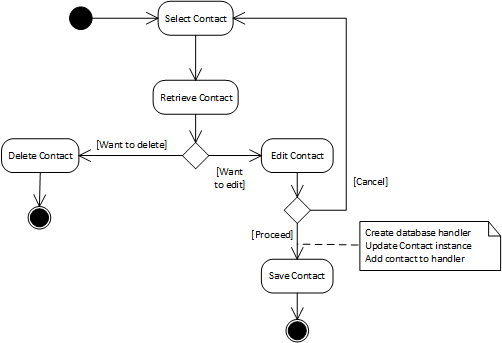
\includegraphics[width=13cm]{diagrams/StateDiagrams/EditContactStateDiagram.png}
\item{Synchronise Contact : FRQ12}\\
\textbf{(Source: Group Deliberation, Priority: High)}
\begin{itemize}
\item The user must be able to synchronize with a contact, at any time, after the contact has been added to the application
\end{itemize}
 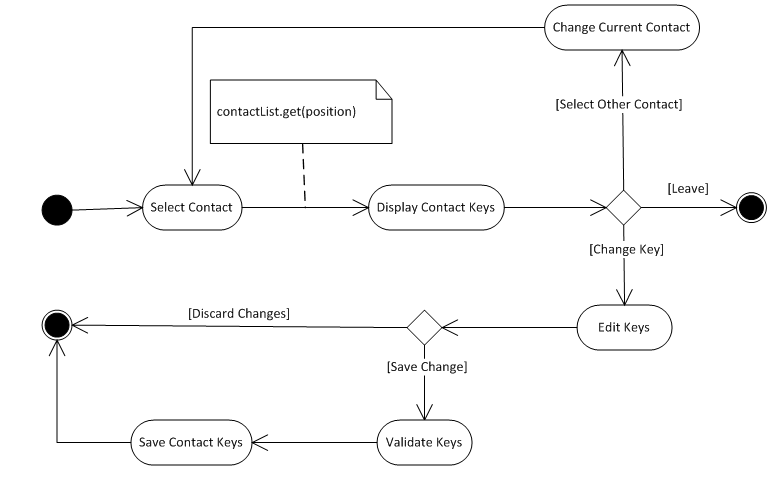
\includegraphics[width=13cm]{diagrams/StateDiagrams/SynchroniseContactState.png}
\item{Remove Contact : FRQ13}\\
\textbf{(Source: Bernard Wagner, Priority: High)}
\begin{itemize}
\item A user must be able to remove an already added contact
\end{itemize}
 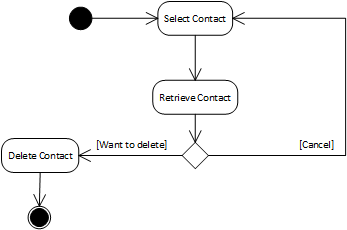
\includegraphics[width=11cm]{diagrams/StateDiagrams/RemoveContactStateDiagram.png}
\end{itemize}

\subsection{Performance requirements}
\begin{itemize}
\item The application should operate in a timely manner. The user should not be made to wait an unreasonable amount of time (this variable can be affected by the system environment e.g. resource availability)
\begin{itemize}
\item The application is expected to encrypt a message in less than one second
\item The application is expected to decrypt a message in less than one second
\end{itemize}
\item The encryption method used must ensure secure communication via compromised communication methods
\begin{itemize}
\item The encyprion method used should have an entropy value of less than 1\%
\end{itemize}
\item The applcaiton must make use of local authentication
\begin{itemize}
\item A user's password must always remain masked; when logging in, or even when editing the user account details
\item A user's password should be encrypted or stored as a hash value within the application database
\item Contact information stored by the application must not be obtainable by unauthorized users
\item Contact information should be encrypted to ensure that it is not readable by unauthorized users
\end{itemize}
\end{itemize}

\subsection{Logical database requirements}

\begin{itemize}
\item The user's password must be hashed using a SHA-256 hash function
\item The data stored by the application should only be viewable by an authorised user
\item Contact data must be encrypted to ensure confidentiality - using an applicable hash function
\item Every user has zero or more contacts associated with it
\item Once a user account is deleted, all data associated with that account, including all saved contacts, will be deleted
\end{itemize}
\begin{center}
 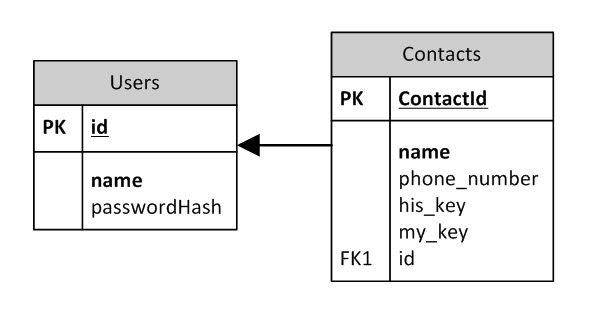
\includegraphics[width=13cm]{diagrams/LogicalDatabase.png}
\end{center}

\subsection{Design constraints}
\begin{itemize}
\item{Message length : DC1}\\
\textbf{(Source: Bernard Wagner, Priority: High)}
\begin{itemize}
\item Due to the fact that the primary messaging service that the client intends to use is SMS, the amount of characters per message is limited to 160 characters in total
\item The encryption process uses 6 characters for a failsafe, and 10 characters to embed the next key to be used for future communication
\item This means that plaintext entered by the user is limited to 144 characters
\item To maintain consistency, we enforce this as the maximum length of messages which the application can encrypt, regardless of the messaging application used to send the message
\end{itemize}
\item{The usable characters : DC2}\\
\textbf{(Source: Bernard Wagner, Priority: High)}
\begin{itemize}
\item The usable characters that can be encrypted by the application is limited to the GSM character set, because the primary messaging service that this application is developed for is SMS.
\end{itemize}
\item{Application resource requirementsr : DC3}\\
\textbf{(Source: Bernard Wagner, Priority: High)}
\begin{itemize}
\item The application should function efficiently, with the least amount of resource usage
\end{itemize}
\end{itemize}
\subsubsection{Standards compliance}
\begin{itemize}
\item The application must be secure, as is stipulated in Appendix D: Secure Sesign Principles
\item The application must conform to the Android and iOS respective platform design principles; these can be found in Appendix E, Design principles
\end{itemize}

\subsection{Software system attributes}
\subsubsection{Reliability}
\begin{itemize}
\item The application should run until the user closes it
\item Any information stored by the application should be static and exist as long as the application is open or said information is edited/removed
\item The ciphertext should decrypt back into its original plaintext
\end{itemize}
\subsubsection{Availability}
\begin{itemize}
\item The user should be able to use the application regardless of runtime, and should not be made to wait while the application performs a function
\item The application should not interfere with any other applications that could be running simultaneously on the device
\end{itemize}
\subsubsection{Security}
\begin{itemize}
\item A secure encryption (and decryption) method will be used for the localised application database
\end{itemize}
\subsubsection{Maintainability}
\begin{itemize}
\item The source code should be simplistic, maintainable, and readable/documented
\item The application should not act in unpredictable ways
\end{itemize}
\subsubsection{Portability}
\begin{itemize}
\item The client has requested that different versions of the application be developed to execute on different mobile operating systems: namely Android and iOS
\end{itemize}
